\documentclass[1p]{elsarticle_modified}
%\bibliographystyle{elsarticle-num}

%\usepackage[colorlinks]{hyperref}
%\usepackage{abbrmath_seonhwa} %\Abb, \Ascr, \Acal ,\Abf, \Afrak
\usepackage{amsfonts}
\usepackage{amssymb}
\usepackage{amsmath}
\usepackage{amsthm}
\usepackage{scalefnt}
\usepackage{amsbsy}
\usepackage{kotex}
\usepackage{caption}
\usepackage{subfig}
\usepackage{color}
\usepackage{graphicx}
\usepackage{xcolor} %% white, black, red, green, blue, cyan, magenta, yellow
\usepackage{float}
\usepackage{setspace}
\usepackage{hyperref}

\usepackage{tikz}
\usetikzlibrary{arrows}

\usepackage{multirow}
\usepackage{array} % fixed length table
\usepackage{hhline}

%%%%%%%%%%%%%%%%%%%%%
\makeatletter
\renewcommand*\env@matrix[1][\arraystretch]{%
	\edef\arraystretch{#1}%
	\hskip -\arraycolsep
	\let\@ifnextchar\new@ifnextchar
	\array{*\c@MaxMatrixCols c}}
\makeatother %https://tex.stackexchange.com/questions/14071/how-can-i-increase-the-line-spacing-in-a-matrix
%%%%%%%%%%%%%%%

\usepackage[normalem]{ulem}

\newcommand{\msout}[1]{\ifmmode\text{\sout{\ensuremath{#1}}}\else\sout{#1}\fi}
%SOURCE: \msout is \stkout macro in https://tex.stackexchange.com/questions/20609/strikeout-in-math-mode

\newcommand{\cancel}[1]{
	\ifmmode
	{\color{red}\msout{#1}}
	\else
	{\color{red}\sout{#1}}
	\fi
}

\newcommand{\add}[1]{
	{\color{blue}\uwave{#1}}
}

\newcommand{\replace}[2]{
	\ifmmode
	{\color{red}\msout{#1}}{\color{blue}\uwave{#2}}
	\else
	{\color{red}\sout{#1}}{\color{blue}\uwave{#2}}
	\fi
}

\newcommand{\Sol}{\mathcal{S}} %segment
\newcommand{\D}{D} %diagram
\newcommand{\A}{\mathcal{A}} %arc


%%%%%%%%%%%%%%%%%%%%%%%%%%%%%5 test

\def\sl{\operatorname{\textup{SL}}(2,\Cbb)}
\def\psl{\operatorname{\textup{PSL}}(2,\Cbb)}
\def\quan{\mkern 1mu \triangleright \mkern 1mu}

\theoremstyle{definition}
\newtheorem{thm}{Theorem}[section]
\newtheorem{prop}[thm]{Proposition}
\newtheorem{lem}[thm]{Lemma}
\newtheorem{ques}[thm]{Question}
\newtheorem{cor}[thm]{Corollary}
\newtheorem{defn}[thm]{Definition}
\newtheorem{exam}[thm]{Example}
\newtheorem{rmk}[thm]{Remark}
\newtheorem{alg}[thm]{Algorithm}

\newcommand{\I}{\sqrt{-1}}
\begin{document}

%\begin{frontmatter}
%
%\title{Boundary parabolic representations of knots up to 8 crossings}
%
%%% Group authors per affiliation:
%\author{Yunhi Cho} 
%\address{Department of Mathematics, University of Seoul, Seoul, Korea}
%\ead{yhcho@uos.ac.kr}
%
%
%\author{Seonhwa Kim} %\fnref{s_kim}}
%\address{Center for Geometry and Physics, Institute for Basic Science, Pohang, 37673, Korea}
%\ead{ryeona17@ibs.re.kr}
%
%\author{Hyuk Kim}
%\address{Department of Mathematical Sciences, Seoul National University, Seoul 08826, Korea}
%\ead{hyukkim@snu.ac.kr}
%
%\author{Seokbeom Yoon}
%\address{Department of Mathematical Sciences, Seoul National University, Seoul, 08826,  Korea}
%\ead{sbyoon15@snu.ac.kr}
%
%\begin{abstract}
%We find all boundary parabolic representation of knots up to 8 crossings.
%
%\end{abstract}
%\begin{keyword}
%    \MSC[2010] 57M25 
%\end{keyword}
%
%\end{frontmatter}

%\linenumbers
%\tableofcontents
%
\newcommand\colored[1]{\textcolor{white}{\rule[-0.35ex]{0.8em}{1.4ex}}\kern-0.8em\color{red} #1}%
%\newcommand\colored[1]{\textcolor{white}{ #1}\kern-2.17ex	\textcolor{white}{ #1}\kern-1.81ex	\textcolor{white}{ #1}\kern-2.15ex\color{red}#1	}

{\Large $\underline{12a_{0949}~(K12a_{0949})}$}

\setlength{\tabcolsep}{10pt}
\renewcommand{\arraystretch}{1.6}
\vspace{1cm}\begin{tabular}{m{100pt}>{\centering\arraybackslash}m{274pt}}
\multirow{5}{120pt}{
	\centering
	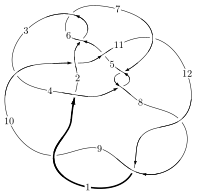
\includegraphics[width=112pt]{../../../GIT/diagram.site/Diagrams/png/1750_12a_0949.png}\\
\ \ \ A knot diagram\footnotemark}&
\allowdisplaybreaks
\textbf{Linearized knot diagam} \\
\cline{2-2}
 &
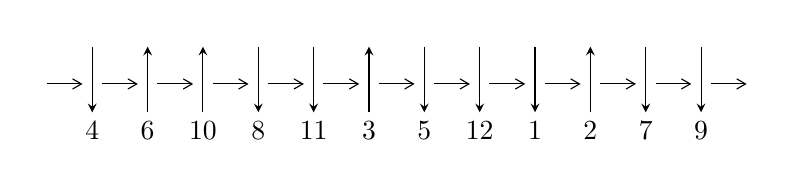
\begin{tikzpicture}[x=20pt, y=17pt]
	% nodes
	\node (C0) at (0, 0) {};
	\node (C1) at (1, 0) {};
	\node (C1U) at (1, +1) {};
	\node (C1D) at (1, -1) {4};

	\node (C2) at (2, 0) {};
	\node (C2U) at (2, +1) {};
	\node (C2D) at (2, -1) {6};

	\node (C3) at (3, 0) {};
	\node (C3U) at (3, +1) {};
	\node (C3D) at (3, -1) {10};

	\node (C4) at (4, 0) {};
	\node (C4U) at (4, +1) {};
	\node (C4D) at (4, -1) {8};

	\node (C5) at (5, 0) {};
	\node (C5U) at (5, +1) {};
	\node (C5D) at (5, -1) {11};

	\node (C6) at (6, 0) {};
	\node (C6U) at (6, +1) {};
	\node (C6D) at (6, -1) {3};

	\node (C7) at (7, 0) {};
	\node (C7U) at (7, +1) {};
	\node (C7D) at (7, -1) {5};

	\node (C8) at (8, 0) {};
	\node (C8U) at (8, +1) {};
	\node (C8D) at (8, -1) {12};

	\node (C9) at (9, 0) {};
	\node (C9U) at (9, +1) {};
	\node (C9D) at (9, -1) {1};

	\node (C10) at (10, 0) {};
	\node (C10U) at (10, +1) {};
	\node (C10D) at (10, -1) {2};

	\node (C11) at (11, 0) {};
	\node (C11U) at (11, +1) {};
	\node (C11D) at (11, -1) {7};

	\node (C12) at (12, 0) {};
	\node (C12U) at (12, +1) {};
	\node (C12D) at (12, -1) {9};
	\node (C13) at (13, 0) {};

	% arrows
	\draw[->,>={angle 60}]
	(C0) edge (C1) (C1) edge (C2) (C2) edge (C3) (C3) edge (C4) (C4) edge (C5) (C5) edge (C6) (C6) edge (C7) (C7) edge (C8) (C8) edge (C9) (C9) edge (C10) (C10) edge (C11) (C11) edge (C12) (C12) edge (C13) ;	\draw[->,>=stealth]
	(C1U) edge (C1D) (C2D) edge (C2U) (C3D) edge (C3U) (C4U) edge (C4D) (C5U) edge (C5D) (C6D) edge (C6U) (C7U) edge (C7D) (C8U) edge (C8D) (C9U) edge (C9D) (C10D) edge (C10U) (C11U) edge (C11D) (C12U) edge (C12D) ;
	\end{tikzpicture} \\
\hhline{~~} \\& 
\textbf{Solving Sequence} \\ \cline{2-2} 
 &
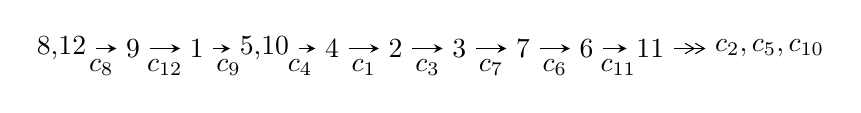
\begin{tikzpicture}[x=23pt, y=7pt]
	% node
	\node (A0) at (-1/8, 0) {8,12};
	\node (A1) at (1, 0) {9};
	\node (A2) at (2, 0) {1};
	\node (A3) at (49/16, 0) {5,10};
	\node (A4) at (33/8, 0) {4};
	\node (A5) at (41/8, 0) {2};
	\node (A6) at (49/8, 0) {3};
	\node (A7) at (57/8, 0) {7};
	\node (A8) at (65/8, 0) {6};
	\node (A9) at (73/8, 0) {11};
	\node (C1) at (1/2, -1) {$c_{8}$};
	\node (C2) at (3/2, -1) {$c_{12}$};
	\node (C3) at (5/2, -1) {$c_{9}$};
	\node (C4) at (29/8, -1) {$c_{4}$};
	\node (C5) at (37/8, -1) {$c_{1}$};
	\node (C6) at (45/8, -1) {$c_{3}$};
	\node (C7) at (53/8, -1) {$c_{7}$};
	\node (C8) at (61/8, -1) {$c_{6}$};
	\node (C9) at (69/8, -1) {$c_{11}$};
	\node (A10) at (11, 0) {$c_{2},c_{5},c_{10}$};

	% edge
	\draw[->,>=stealth]	
	(A0) edge (A1) (A1) edge (A2) (A2) edge (A3) (A3) edge (A4) (A4) edge (A5) (A5) edge (A6) (A6) edge (A7) (A7) edge (A8) (A8) edge (A9) ;
	\draw[->>,>={angle 60}]	
	(A9) edge (A10);
\end{tikzpicture} \\ 

\end{tabular} \\

\footnotetext{
The image of knot diagram is generated by the software ``\textbf{Draw programme}" developed by Andrew Bartholomew(\url{http://www.layer8.co.uk/maths/draw/index.htm\#Running-draw}), where we modified some parts for our purpose(\url{https://github.com/CATsTAILs/LinksPainter}).
}\phantom \\ \newline 
\centering \textbf{Ideals for irreducible components\footnotemark of $X_{\text{par}}$} 
 
\begin{align*}
I^u_{1}&=\langle 
-2.31639\times10^{422} u^{132}+1.53310\times10^{423} u^{131}+\cdots+1.77653\times10^{424} b+1.30059\times10^{424},\\
\phantom{I^u_{1}}&\phantom{= \langle  }-3.70487\times10^{424} u^{132}+1.90525\times10^{425} u^{131}+\cdots+2.13183\times10^{424} a+4.70733\times10^{425},\\
\phantom{I^u_{1}}&\phantom{= \langle  }u^{133}-5 u^{132}+\cdots-56 u-3\rangle \\
I^u_{2}&=\langle 
6761534 u^{24}+25064228 u^{23}+\cdots+32603 b-5175546,\\
\phantom{I^u_{2}}&\phantom{= \langle  }-3451225 u^{24}-12321594 u^{23}+\cdots+32603 a+2498173,\;u^{25}+5 u^{24}+\cdots-7 u-1\rangle \\
I^u_{3}&=\langle 
-6 a^3+2 a^2+b-27 a-9,\;2 a^4+9 a^2+6 a+1,\;u-1\rangle \\
I^u_{4}&=\langle 
b,\;a-1,\;u-1\rangle \\
\\
\end{align*}
\raggedright * 4 irreducible components of $\dim_{\mathbb{C}}=0$, with total 163 representations.\\
\footnotetext{All coefficients of polynomials are rational numbers. But the coefficients are sometimes approximated in decimal forms when there is not enough margin.}
\newpage
\renewcommand{\arraystretch}{1}
\centering \section*{I. $I^u_{1}= \langle -2.32\times10^{422} u^{132}+1.53\times10^{423} u^{131}+\cdots+1.78\times10^{424} b+1.30\times10^{424},\;-3.70\times10^{424} u^{132}+1.91\times10^{425} u^{131}+\cdots+2.13\times10^{424} a+4.71\times10^{425},\;u^{133}-5 u^{132}+\cdots-56 u-3 \rangle$}
\flushleft \textbf{(i) Arc colorings}\\
\begin{tabular}{m{7pt} m{180pt} m{7pt} m{180pt} }
\flushright $a_{8}=$&$\begin{pmatrix}1\\0\end{pmatrix}$ \\
\flushright $a_{12}=$&$\begin{pmatrix}0\\u\end{pmatrix}$ \\
\flushright $a_{9}=$&$\begin{pmatrix}1\\u^2\end{pmatrix}$ \\
\flushright $a_{1}=$&$\begin{pmatrix}- u\\- u^3+u\end{pmatrix}$ \\
\flushright $a_{5}=$&$\begin{pmatrix}1.73788 u^{132}-8.93715 u^{131}+\cdots-298.967 u-22.0812\\0.0130389 u^{132}-0.0862979 u^{131}+\cdots-11.5157 u-0.732099\end{pmatrix}$ \\
\flushright $a_{10}=$&$\begin{pmatrix}- u^2+1\\- u^4+2 u^2\end{pmatrix}$ \\
\flushright $a_{4}=$&$\begin{pmatrix}1.75092 u^{132}-9.02344 u^{131}+\cdots-310.482 u-22.8133\\0.0130389 u^{132}-0.0862979 u^{131}+\cdots-11.5157 u-0.732099\end{pmatrix}$ \\
\flushright $a_{2}=$&$\begin{pmatrix}-1.63049 u^{132}+8.15688 u^{131}+\cdots+595.484 u+44.4192\\0.356925 u^{132}-1.97497 u^{131}+\cdots-21.3742 u-0.805447\end{pmatrix}$ \\
\flushright $a_{3}=$&$\begin{pmatrix}1.81952 u^{132}-9.36921 u^{131}+\cdots-327.425 u-24.1733\\0.000295256 u^{132}-0.0526861 u^{131}+\cdots-14.0734 u-0.887146\end{pmatrix}$ \\
\flushright $a_{7}=$&$\begin{pmatrix}0.0524645 u^{132}-0.199611 u^{131}+\cdots-69.0014 u-6.56518\\-0.0372953 u^{132}+0.479760 u^{131}+\cdots+8.11647 u+0.646970\end{pmatrix}$ \\
\flushright $a_{6}=$&$\begin{pmatrix}0.956137 u^{132}-4.71492 u^{131}+\cdots-444.889 u-30.0851\\-0.322208 u^{132}+1.81509 u^{131}+\cdots+5.03229 u-0.932874\end{pmatrix}$ \\
\flushright $a_{11}=$&$\begin{pmatrix}-3.25930 u^{132}+16.4774 u^{131}+\cdots+738.406 u+42.2610\\-0.130790 u^{132}+0.834469 u^{131}+\cdots+87.2420 u+6.33965\end{pmatrix}$\\&\end{tabular}
\flushleft \textbf{(ii) Obstruction class $= -1$}\\~\\
\flushleft \textbf{(iii) Cusp Shapes $= 1.17653 u^{132}-5.26495 u^{131}+\cdots-634.853 u-55.6689$}\\~\\
\newpage\renewcommand{\arraystretch}{1}
\flushleft \textbf{(iv) u-Polynomials at the component}\newline \\
\begin{tabular}{m{50pt}|m{274pt}}
Crossings & \hspace{64pt}u-Polynomials at each crossing \\
\hline $$\begin{aligned}c_{1}\end{aligned}$$&$\begin{aligned}
&u^{133}-15 u^{132}+\cdots+11068 u-1172
\end{aligned}$\\
\hline $$\begin{aligned}c_{2},c_{6}\end{aligned}$$&$\begin{aligned}
&u^{133}-3 u^{132}+\cdots-17081 u+1539
\end{aligned}$\\
\hline $$\begin{aligned}c_{3}\end{aligned}$$&$\begin{aligned}
&2(2 u^{133}+2 u^{132}+\cdots+11264 u+2048)
\end{aligned}$\\
\hline $$\begin{aligned}c_{4},c_{7}\end{aligned}$$&$\begin{aligned}
&u^{133}-9 u^{132}+\cdots-24896 u+1952
\end{aligned}$\\
\hline $$\begin{aligned}c_{5}\end{aligned}$$&$\begin{aligned}
&2(2 u^{133}+2 u^{132}+\cdots+7848686 u+3253981)
\end{aligned}$\\
\hline $$\begin{aligned}c_{8},c_{9},c_{12}\end{aligned}$$&$\begin{aligned}
&u^{133}+5 u^{132}+\cdots-56 u+3
\end{aligned}$\\
\hline $$\begin{aligned}c_{10}\end{aligned}$$&$\begin{aligned}
&u^{133}+7 u^{132}+\cdots+62070 u+9146
\end{aligned}$\\
\hline $$\begin{aligned}c_{11}\end{aligned}$$&$\begin{aligned}
&u^{133}+7 u^{130}+\cdots+14366 u+3254
\end{aligned}$\\
\hline
\end{tabular}\\~\\
\newpage\renewcommand{\arraystretch}{1}
\flushleft \textbf{(v) Riley Polynomials at the component}\newline \\
\begin{tabular}{m{50pt}|m{274pt}}
Crossings & \hspace{64pt}Riley Polynomials at each crossing \\
\hline $$\begin{aligned}c_{1}\end{aligned}$$&$\begin{aligned}
&y^{133}-7 y^{132}+\cdots-104928320 y-1373584
\end{aligned}$\\
\hline $$\begin{aligned}c_{2},c_{6}\end{aligned}$$&$\begin{aligned}
&y^{133}-77 y^{132}+\cdots+162555355 y-2368521
\end{aligned}$\\
\hline $$\begin{aligned}c_{3}\end{aligned}$$&$\begin{aligned}
&4(4 y^{133}+192 y^{132}+\cdots-1.10100\times10^{8} y-4194304)
\end{aligned}$\\
\hline $$\begin{aligned}c_{4},c_{7}\end{aligned}$$&$\begin{aligned}
&y^{133}+93 y^{132}+\cdots-337168896 y-3810304
\end{aligned}$\\
\hline $$\begin{aligned}c_{5}\end{aligned}$$&$\begin{aligned}
&4(4 y^{133}+240 y^{132}+\cdots-5.32285\times10^{14} y-1.05884\times10^{13})
\end{aligned}$\\
\hline $$\begin{aligned}c_{8},c_{9},c_{12}\end{aligned}$$&$\begin{aligned}
&y^{133}-137 y^{132}+\cdots-56 y-9
\end{aligned}$\\
\hline $$\begin{aligned}c_{10}\end{aligned}$$&$\begin{aligned}
&y^{133}-51 y^{132}+\cdots+15173548824 y-83649316
\end{aligned}$\\
\hline $$\begin{aligned}c_{11}\end{aligned}$$&$\begin{aligned}
&y^{133}+108 y^{131}+\cdots-2741332040 y-10588516
\end{aligned}$\\
\hline
\end{tabular}\\~\\
\newpage\flushleft \textbf{(vi) Complex Volumes and Cusp Shapes}
$$\begin{array}{c|c|c}  
\text{Solutions to }I^u_{1}& \I (\text{vol} + \sqrt{-1}CS) & \text{Cusp shape}\\
 \hline 
\begin{aligned}
u &= -0.574211 + 0.806522 I \\
a &= -0.47135 - 1.68203 I \\
b &= -0.458336 + 1.314170 I\end{aligned}
 & \phantom{-}2.92527 + 8.52139 I & \phantom{-0.000000 } 0 \\ \hline\begin{aligned}
u &= -0.574211 - 0.806522 I \\
a &= -0.47135 + 1.68203 I \\
b &= -0.458336 - 1.314170 I\end{aligned}
 & \phantom{-}2.92527 - 8.52139 I & \phantom{-0.000000 } 0 \\ \hline\begin{aligned}
u &= \phantom{-}0.378103 + 0.906879 I \\
a &= \phantom{-}0.33971 - 2.11105 I \\
b &= \phantom{-}0.293973 + 1.167940 I\end{aligned}
 & \phantom{-}2.16623 - 4.99446 I & \phantom{-0.000000 } 0 \\ \hline\begin{aligned}
u &= \phantom{-}0.378103 - 0.906879 I \\
a &= \phantom{-}0.33971 + 2.11105 I \\
b &= \phantom{-}0.293973 - 1.167940 I\end{aligned}
 & \phantom{-}2.16623 + 4.99446 I & \phantom{-0.000000 } 0 \\ \hline\begin{aligned}
u &= \phantom{-}0.329684 + 0.964221 I \\
a &= \phantom{-}0.01448 + 1.45443 I \\
b &= -0.445410 - 0.888166 I\end{aligned}
 & \phantom{-}1.46652 - 5.73875 I & \phantom{-0.000000 } 0 \\ \hline\begin{aligned}
u &= \phantom{-}0.329684 - 0.964221 I \\
a &= \phantom{-}0.01448 - 1.45443 I \\
b &= -0.445410 + 0.888166 I\end{aligned}
 & \phantom{-}1.46652 + 5.73875 I & \phantom{-0.000000 } 0 \\ \hline\begin{aligned}
u &= -0.494919 + 0.893036 I \\
a &= \phantom{-}0.71500 + 1.26830 I \\
b &= -0.238880 - 1.154660 I\end{aligned}
 & \phantom{-}3.16581 - 3.01226 I & \phantom{-0.000000 } 0 \\ \hline\begin{aligned}
u &= -0.494919 - 0.893036 I \\
a &= \phantom{-}0.71500 - 1.26830 I \\
b &= -0.238880 + 1.154660 I\end{aligned}
 & \phantom{-}3.16581 + 3.01226 I & \phantom{-0.000000 } 0 \\ \hline\begin{aligned}
u &= \phantom{-}0.924375 + 0.465795 I \\
a &= \phantom{-}0.341741 - 0.191628 I \\
b &= -0.437473 + 0.302466 I\end{aligned}
 & -0.783926 + 0.529519 I & \phantom{-0.000000 } 0 \\ \hline\begin{aligned}
u &= \phantom{-}0.924375 - 0.465795 I \\
a &= \phantom{-}0.341741 + 0.191628 I \\
b &= -0.437473 - 0.302466 I\end{aligned}
 & -0.783926 - 0.529519 I & \phantom{-0.000000 } 0\\
 \hline 
 \end{array}$$\newpage$$\begin{array}{c|c|c}  
\text{Solutions to }I^u_{1}& \I (\text{vol} + \sqrt{-1}CS) & \text{Cusp shape}\\
 \hline 
\begin{aligned}
u &= \phantom{-}1.014880 + 0.249045 I \\
a &= \phantom{-}0.26982 - 2.02091 I \\
b &= \phantom{-}0.025828 + 1.409670 I\end{aligned}
 & \phantom{-}4.71692 + 1.38176 I & \phantom{-0.000000 } 0 \\ \hline\begin{aligned}
u &= \phantom{-}1.014880 - 0.249045 I \\
a &= \phantom{-}0.26982 + 2.02091 I \\
b &= \phantom{-}0.025828 - 1.409670 I\end{aligned}
 & \phantom{-}4.71692 - 1.38176 I & \phantom{-0.000000 } 0 \\ \hline\begin{aligned}
u &= \phantom{-}0.373883 + 0.866496 I \\
a &= -0.02527 + 1.93367 I \\
b &= -0.332906 - 1.081600 I\end{aligned}
 & \phantom{-}1.43426 - 2.64312 I & \phantom{-0.000000 } 0 \\ \hline\begin{aligned}
u &= \phantom{-}0.373883 - 0.866496 I \\
a &= -0.02527 - 1.93367 I \\
b &= -0.332906 + 1.081600 I\end{aligned}
 & \phantom{-}1.43426 + 2.64312 I & \phantom{-0.000000 } 0 \\ \hline\begin{aligned}
u &= -0.532921 + 0.915024 I \\
a &= \phantom{-}0.33759 + 1.80539 I \\
b &= \phantom{-}0.482952 - 1.319860 I\end{aligned}
 & \phantom{-}6.2072 + 14.4323 I & \phantom{-0.000000 } 0 \\ \hline\begin{aligned}
u &= -0.532921 - 0.915024 I \\
a &= \phantom{-}0.33759 - 1.80539 I \\
b &= \phantom{-}0.482952 + 1.319860 I\end{aligned}
 & \phantom{-}6.2072 - 14.4323 I & \phantom{-0.000000 } 0 \\ \hline\begin{aligned}
u &= \phantom{-}0.989465 + 0.379484 I \\
a &= -0.80123 + 1.55516 I \\
b &= \phantom{-}0.091704 - 0.713483 I\end{aligned}
 & \phantom{-}0.263606 - 0.184369 I & \phantom{-0.000000 } 0 \\ \hline\begin{aligned}
u &= \phantom{-}0.989465 - 0.379484 I \\
a &= -0.80123 - 1.55516 I \\
b &= \phantom{-}0.091704 + 0.713483 I\end{aligned}
 & \phantom{-}0.263606 + 0.184369 I & \phantom{-0.000000 } 0 \\ \hline\begin{aligned}
u &= \phantom{-}0.415346 + 0.990925 I \\
a &= \phantom{-}0.386696 - 1.313430 I \\
b &= \phantom{-}0.157988 + 0.867765 I\end{aligned}
 & \phantom{-}0.46372 - 2.33810 I & \phantom{-0.000000 } 0 \\ \hline\begin{aligned}
u &= \phantom{-}0.415346 - 0.990925 I \\
a &= \phantom{-}0.386696 + 1.313430 I \\
b &= \phantom{-}0.157988 - 0.867765 I\end{aligned}
 & \phantom{-}0.46372 + 2.33810 I & \phantom{-0.000000 } 0\\
 \hline 
 \end{array}$$\newpage$$\begin{array}{c|c|c}  
\text{Solutions to }I^u_{1}& \I (\text{vol} + \sqrt{-1}CS) & \text{Cusp shape}\\
 \hline 
\begin{aligned}
u &= \phantom{-}0.704660 + 0.550275 I \\
a &= \phantom{-}1.200850 - 0.552040 I \\
b &= -0.097070 + 1.128250 I\end{aligned}
 & \phantom{-}2.06026 - 1.40425 I & \phantom{-0.000000 } 0 \\ \hline\begin{aligned}
u &= \phantom{-}0.704660 - 0.550275 I \\
a &= \phantom{-}1.200850 + 0.552040 I \\
b &= -0.097070 - 1.128250 I\end{aligned}
 & \phantom{-}2.06026 + 1.40425 I & \phantom{-0.000000 } 0 \\ \hline\begin{aligned}
u &= -0.696078 + 0.514809 I \\
a &= -0.723227 - 0.979580 I \\
b &= \phantom{-}0.215798 + 1.326840 I\end{aligned}
 & \phantom{-}7.58706 + 0.38056 I & \phantom{-0.000000 } 0 \\ \hline\begin{aligned}
u &= -0.696078 - 0.514809 I \\
a &= -0.723227 + 0.979580 I \\
b &= \phantom{-}0.215798 - 1.326840 I\end{aligned}
 & \phantom{-}7.58706 - 0.38056 I & \phantom{-0.000000 } 0 \\ \hline\begin{aligned}
u &= \phantom{-}0.566105 + 0.614307 I \\
a &= -0.0235346 - 0.0690271 I \\
b &= \phantom{-}0.441384 - 0.059551 I\end{aligned}
 & -1.03448 - 2.04846 I & \phantom{-0.000000 } 0 \\ \hline\begin{aligned}
u &= \phantom{-}0.566105 - 0.614307 I \\
a &= -0.0235346 + 0.0690271 I \\
b &= \phantom{-}0.441384 + 0.059551 I\end{aligned}
 & -1.03448 + 2.04846 I & \phantom{-0.000000 } 0 \\ \hline\begin{aligned}
u &= \phantom{-}0.794351 + 0.230141 I \\
a &= -0.43059 + 1.98792 I \\
b &= \phantom{-}0.204220 - 0.503604 I\end{aligned}
 & \phantom{-}0.237202 - 0.167348 I & \phantom{-0.000000 } 0 \\ \hline\begin{aligned}
u &= \phantom{-}0.794351 - 0.230141 I \\
a &= -0.43059 - 1.98792 I \\
b &= \phantom{-}0.204220 + 0.503604 I\end{aligned}
 & \phantom{-}0.237202 + 0.167348 I & \phantom{-0.000000 } 0 \\ \hline\begin{aligned}
u &= \phantom{-}1.109050 + 0.393892 I \\
a &= -0.521767 + 0.393448 I \\
b &= \phantom{-}0.343256 - 1.259130 I\end{aligned}
 & \phantom{-}4.40836 + 2.54732 I & \phantom{-0.000000 } 0 \\ \hline\begin{aligned}
u &= \phantom{-}1.109050 - 0.393892 I \\
a &= -0.521767 - 0.393448 I \\
b &= \phantom{-}0.343256 + 1.259130 I\end{aligned}
 & \phantom{-}4.40836 - 2.54732 I & \phantom{-0.000000 } 0\\
 \hline 
 \end{array}$$\newpage$$\begin{array}{c|c|c}  
\text{Solutions to }I^u_{1}& \I (\text{vol} + \sqrt{-1}CS) & \text{Cusp shape}\\
 \hline 
\begin{aligned}
u &= -0.403984 + 0.683130 I \\
a &= \phantom{-}0.84329 + 1.84290 I \\
b &= \phantom{-}0.417585 - 1.322650 I\end{aligned}
 & \phantom{-}8.44013 + 3.83414 I & \phantom{-0.000000 } 0 \\ \hline\begin{aligned}
u &= -0.403984 - 0.683130 I \\
a &= \phantom{-}0.84329 - 1.84290 I \\
b &= \phantom{-}0.417585 + 1.322650 I\end{aligned}
 & \phantom{-}8.44013 - 3.83414 I & \phantom{-0.000000 } 0 \\ \hline\begin{aligned}
u &= -0.537463 + 0.563850 I \\
a &= -0.450237 + 0.016524 I \\
b &= \phantom{-}0.964956 - 0.103893 I\end{aligned}
 & \phantom{-}1.89345 + 9.32259 I & \phantom{-0.000000 } 0 \\ \hline\begin{aligned}
u &= -0.537463 - 0.563850 I \\
a &= -0.450237 - 0.016524 I \\
b &= \phantom{-}0.964956 + 0.103893 I\end{aligned}
 & \phantom{-}1.89345 - 9.32259 I & \phantom{-0.000000 } 0 \\ \hline\begin{aligned}
u &= -0.727912 + 0.988878 I \\
a &= -0.651866 - 1.171610 I \\
b &= \phantom{-}0.320963 + 1.149250 I\end{aligned}
 & \phantom{-}5.78280 - 8.24577 I & \phantom{-0.000000 } 0 \\ \hline\begin{aligned}
u &= -0.727912 - 0.988878 I \\
a &= -0.651866 + 1.171610 I \\
b &= \phantom{-}0.320963 - 1.149250 I\end{aligned}
 & \phantom{-}5.78280 + 8.24577 I & \phantom{-0.000000 } 0 \\ \hline\begin{aligned}
u &= -0.224218 + 0.729839 I \\
a &= -0.653937 + 1.176690 I \\
b &= \phantom{-}0.355795 - 0.141174 I\end{aligned}
 & \phantom{-}2.87171 - 5.33242 I & \phantom{-0.000000 } 0 \\ \hline\begin{aligned}
u &= -0.224218 - 0.729839 I \\
a &= -0.653937 - 1.176690 I \\
b &= \phantom{-}0.355795 + 0.141174 I\end{aligned}
 & \phantom{-}2.87171 + 5.33242 I & \phantom{-0.000000 } 0 \\ \hline\begin{aligned}
u &= \phantom{-}0.497368 + 0.554874 I \\
a &= \phantom{-}0.613055 - 1.117160 I \\
b &= -0.633997 + 0.494336 I\end{aligned}
 & \phantom{-}0.34427 - 1.51811 I & \phantom{-0.000000 } 0 \\ \hline\begin{aligned}
u &= \phantom{-}0.497368 - 0.554874 I \\
a &= \phantom{-}0.613055 + 1.117160 I \\
b &= -0.633997 - 0.494336 I\end{aligned}
 & \phantom{-}0.34427 + 1.51811 I & \phantom{-0.000000 } 0\\
 \hline 
 \end{array}$$\newpage$$\begin{array}{c|c|c}  
\text{Solutions to }I^u_{1}& \I (\text{vol} + \sqrt{-1}CS) & \text{Cusp shape}\\
 \hline 
\begin{aligned}
u &= \phantom{-}0.114871 + 0.720135 I \\
a &= -0.03182 - 1.98080 I \\
b &= \phantom{-}0.550237 + 1.300370 I\end{aligned}
 & \phantom{-}7.41576 - 6.58321 I & \phantom{-0.000000 } 0 \\ \hline\begin{aligned}
u &= \phantom{-}0.114871 - 0.720135 I \\
a &= -0.03182 + 1.98080 I \\
b &= \phantom{-}0.550237 - 1.300370 I\end{aligned}
 & \phantom{-}7.41576 + 6.58321 I & \phantom{-0.000000 } 0 \\ \hline\begin{aligned}
u &= \phantom{-}0.351793 + 0.590951 I \\
a &= -0.10506 + 1.82082 I \\
b &= -0.360927 - 1.349490 I\end{aligned}
 & \phantom{-}3.01841 - 2.63877 I & \phantom{-0.000000 } 0 \\ \hline\begin{aligned}
u &= \phantom{-}0.351793 - 0.590951 I \\
a &= -0.10506 - 1.82082 I \\
b &= -0.360927 + 1.349490 I\end{aligned}
 & \phantom{-}3.01841 + 2.63877 I & \phantom{-0.000000 } 0 \\ \hline\begin{aligned}
u &= -1.327140 + 0.014584 I \\
a &= -1.88231 + 0.42302 I \\
b &= -0.053802 - 0.861572 I\end{aligned}
 & \phantom{-}0.47041 + 6.74381 I & \phantom{-0.000000 } 0 \\ \hline\begin{aligned}
u &= -1.327140 - 0.014584 I \\
a &= -1.88231 - 0.42302 I \\
b &= -0.053802 + 0.861572 I\end{aligned}
 & \phantom{-}0.47041 - 6.74381 I & \phantom{-0.000000 } 0 \\ \hline\begin{aligned}
u &= \phantom{-}0.262945 + 0.616414 I \\
a &= -2.10232 + 2.36683 I \\
b &= \phantom{-}0.015632 - 1.219980 I\end{aligned}
 & \phantom{-}6.85021 - 4.66073 I & \phantom{-0.000000 } 0 \\ \hline\begin{aligned}
u &= \phantom{-}0.262945 - 0.616414 I \\
a &= -2.10232 - 2.36683 I \\
b &= \phantom{-}0.015632 + 1.219980 I\end{aligned}
 & \phantom{-}6.85021 + 4.66073 I & \phantom{-0.000000 } 0 \\ \hline\begin{aligned}
u &= \phantom{-}1.329540 + 0.095124 I \\
a &= \phantom{-}0.929518 - 0.191850 I \\
b &= \phantom{-}1.000780 - 0.423256 I\end{aligned}
 & -0.607150 - 1.109740 I & \phantom{-0.000000 } 0 \\ \hline\begin{aligned}
u &= \phantom{-}1.329540 - 0.095124 I \\
a &= \phantom{-}0.929518 + 0.191850 I \\
b &= \phantom{-}1.000780 + 0.423256 I\end{aligned}
 & -0.607150 + 1.109740 I & \phantom{-0.000000 } 0\\
 \hline 
 \end{array}$$\newpage$$\begin{array}{c|c|c}  
\text{Solutions to }I^u_{1}& \I (\text{vol} + \sqrt{-1}CS) & \text{Cusp shape}\\
 \hline 
\begin{aligned}
u &= -1.333530 + 0.040329 I \\
a &= \phantom{-}0.587200 + 0.036810 I \\
b &= \phantom{-}1.35622 - 1.13947 I\end{aligned}
 & \phantom{-}1.19011 - 1.90299 I & \phantom{-0.000000 } 0 \\ \hline\begin{aligned}
u &= -1.333530 - 0.040329 I \\
a &= \phantom{-}0.587200 - 0.036810 I \\
b &= \phantom{-}1.35622 + 1.13947 I\end{aligned}
 & \phantom{-}1.19011 + 1.90299 I & \phantom{-0.000000 } 0 \\ \hline\begin{aligned}
u &= -1.333000 + 0.230008 I \\
a &= \phantom{-}1.054960 + 0.765005 I \\
b &= \phantom{-}0.81399 - 1.29343 I\end{aligned}
 & \phantom{-}2.88699 + 9.95019 I & \phantom{-0.000000 } 0 \\ \hline\begin{aligned}
u &= -1.333000 - 0.230008 I \\
a &= \phantom{-}1.054960 - 0.765005 I \\
b &= \phantom{-}0.81399 + 1.29343 I\end{aligned}
 & \phantom{-}2.88699 - 9.95019 I & \phantom{-0.000000 } 0 \\ \hline\begin{aligned}
u &= \phantom{-}1.341420 + 0.193854 I \\
a &= \phantom{-}0.903653 - 0.557086 I \\
b &= \phantom{-}0.275026 + 0.815619 I\end{aligned}
 & -1.95121 - 1.33658 I & \phantom{-0.000000 } 0 \\ \hline\begin{aligned}
u &= \phantom{-}1.341420 - 0.193854 I \\
a &= \phantom{-}0.903653 + 0.557086 I \\
b &= \phantom{-}0.275026 - 0.815619 I\end{aligned}
 & -1.95121 + 1.33658 I & \phantom{-0.000000 } 0 \\ \hline\begin{aligned}
u &= \phantom{-}1.358650 + 0.106966 I \\
a &= -0.904994 - 0.219653 I \\
b &= -0.194170 - 1.017110 I\end{aligned}
 & \phantom{-}1.65394 - 1.39071 I & \phantom{-0.000000 } 0 \\ \hline\begin{aligned}
u &= \phantom{-}1.358650 - 0.106966 I \\
a &= -0.904994 + 0.219653 I \\
b &= -0.194170 + 1.017110 I\end{aligned}
 & \phantom{-}1.65394 + 1.39071 I & \phantom{-0.000000 } 0 \\ \hline\begin{aligned}
u &= -0.592092 + 0.221364 I \\
a &= \phantom{-}0.052072 + 1.246130 I \\
b &= \phantom{-}0.662794 + 0.347988 I\end{aligned}
 & \phantom{-}2.24208 + 3.37065 I & -4.00000 - 5.75675 I \\ \hline\begin{aligned}
u &= -0.592092 - 0.221364 I \\
a &= \phantom{-}0.052072 - 1.246130 I \\
b &= \phantom{-}0.662794 - 0.347988 I\end{aligned}
 & \phantom{-}2.24208 - 3.37065 I & -4.00000 + 5.75675 I\\
 \hline 
 \end{array}$$\newpage$$\begin{array}{c|c|c}  
\text{Solutions to }I^u_{1}& \I (\text{vol} + \sqrt{-1}CS) & \text{Cusp shape}\\
 \hline 
\begin{aligned}
u &= \phantom{-}1.371290 + 0.051878 I \\
a &= \phantom{-}0.065385 + 0.438714 I \\
b &= \phantom{-}0.61251 - 2.18568 I\end{aligned}
 & \phantom{-}0.93911 - 3.98308 I & \phantom{-0.000000 } 0 \\ \hline\begin{aligned}
u &= \phantom{-}1.371290 - 0.051878 I \\
a &= \phantom{-}0.065385 - 0.438714 I \\
b &= \phantom{-}0.61251 + 2.18568 I\end{aligned}
 & \phantom{-}0.93911 + 3.98308 I & \phantom{-0.000000 } 0 \\ \hline\begin{aligned}
u &= -1.372810 + 0.037798 I \\
a &= \phantom{-}0.03694 + 1.45996 I \\
b &= -0.05136 - 1.62620 I\end{aligned}
 & \phantom{-}2.21593 + 0.54322 I & \phantom{-0.000000 } 0 \\ \hline\begin{aligned}
u &= -1.372810 - 0.037798 I \\
a &= \phantom{-}0.03694 - 1.45996 I \\
b &= -0.05136 + 1.62620 I\end{aligned}
 & \phantom{-}2.21593 - 0.54322 I & \phantom{-0.000000 } 0 \\ \hline\begin{aligned}
u &= -0.476540 + 0.391755 I \\
a &= \phantom{-}0.155313 - 0.074410 I \\
b &= -0.987024 + 0.180034 I\end{aligned}
 & -1.57068 + 3.54785 I & -6.35480 - 10.17340 I \\ \hline\begin{aligned}
u &= -0.476540 - 0.391755 I \\
a &= \phantom{-}0.155313 + 0.074410 I \\
b &= -0.987024 - 0.180034 I\end{aligned}
 & -1.57068 - 3.54785 I & -6.35480 + 10.17340 I \\ \hline\begin{aligned}
u &= -1.385030 + 0.101265 I \\
a &= -0.429680 - 1.218680 I \\
b &= -0.302767 + 1.261620 I\end{aligned}
 & -3.45355 + 3.71222 I & \phantom{-0.000000 } 0 \\ \hline\begin{aligned}
u &= -1.385030 - 0.101265 I \\
a &= -0.429680 + 1.218680 I \\
b &= -0.302767 - 1.261620 I\end{aligned}
 & -3.45355 - 3.71222 I & \phantom{-0.000000 } 0 \\ \hline\begin{aligned}
u &= \phantom{-}0.609207\phantom{ +0.000000I} \\
a &= \phantom{-}0.540750\phantom{ +0.000000I} \\
b &= -0.447332\phantom{ +0.000000I}\end{aligned}
 & -1.11415\phantom{ +0.000000I} & -9.92320\phantom{ +0.000000I} \\ \hline\begin{aligned}
u &= -1.404830 + 0.005344 I \\
a &= \phantom{-}1.004270 - 0.956018 I \\
b &= \phantom{-}0.274246 + 0.967774 I\end{aligned}
 & -4.96359 + 2.05422 I & \phantom{-0.000000 } 0\\
 \hline 
 \end{array}$$\newpage$$\begin{array}{c|c|c}  
\text{Solutions to }I^u_{1}& \I (\text{vol} + \sqrt{-1}CS) & \text{Cusp shape}\\
 \hline 
\begin{aligned}
u &= -1.404830 - 0.005344 I \\
a &= \phantom{-}1.004270 + 0.956018 I \\
b &= \phantom{-}0.274246 - 0.967774 I\end{aligned}
 & -4.96359 - 2.05422 I & \phantom{-0.000000 } 0 \\ \hline\begin{aligned}
u &= -1.40742 + 0.14663 I \\
a &= -0.635566 - 0.606471 I \\
b &= -0.85324 + 1.52041 I\end{aligned}
 & -2.53143 + 5.14360 I & \phantom{-0.000000 } 0 \\ \hline\begin{aligned}
u &= -1.40742 - 0.14663 I \\
a &= -0.635566 + 0.606471 I \\
b &= -0.85324 - 1.52041 I\end{aligned}
 & -2.53143 - 5.14360 I & \phantom{-0.000000 } 0 \\ \hline\begin{aligned}
u &= \phantom{-}1.41489 + 0.04091 I \\
a &= -1.101290 + 0.645661 I \\
b &= -0.663322 - 1.121380 I\end{aligned}
 & -5.66604 - 2.49553 I & \phantom{-0.000000 } 0 \\ \hline\begin{aligned}
u &= \phantom{-}1.41489 - 0.04091 I \\
a &= -1.101290 - 0.645661 I \\
b &= -0.663322 + 1.121380 I\end{aligned}
 & -5.66604 + 2.49553 I & \phantom{-0.000000 } 0 \\ \hline\begin{aligned}
u &= \phantom{-}1.43348 + 0.07898 I \\
a &= \phantom{-}1.40726 - 1.33578 I \\
b &= \phantom{-}0.412663 + 1.258010 I\end{aligned}
 & -1.28880 - 8.09029 I & \phantom{-0.000000 } 0 \\ \hline\begin{aligned}
u &= \phantom{-}1.43348 - 0.07898 I \\
a &= \phantom{-}1.40726 + 1.33578 I \\
b &= \phantom{-}0.412663 - 1.258010 I\end{aligned}
 & -1.28880 + 8.09029 I & \phantom{-0.000000 } 0 \\ \hline\begin{aligned}
u &= -1.43702 + 0.20766 I \\
a &= -1.74439 - 0.47596 I \\
b &= -0.131205 + 1.056820 I\end{aligned}
 & \phantom{-}1.32313 + 7.60879 I & \phantom{-0.000000 } 0 \\ \hline\begin{aligned}
u &= -1.43702 - 0.20766 I \\
a &= -1.74439 + 0.47596 I \\
b &= -0.131205 - 1.056820 I\end{aligned}
 & \phantom{-}1.32313 - 7.60879 I & \phantom{-0.000000 } 0 \\ \hline\begin{aligned}
u &= -0.135763 + 0.492747 I \\
a &= -0.419702 + 0.679952 I \\
b &= \phantom{-}0.980114 - 0.157893 I\end{aligned}
 & \phantom{-}3.83136 - 0.94632 I & \phantom{-}3.69353 - 2.08963 I\\
 \hline 
 \end{array}$$\newpage$$\begin{array}{c|c|c}  
\text{Solutions to }I^u_{1}& \I (\text{vol} + \sqrt{-1}CS) & \text{Cusp shape}\\
 \hline 
\begin{aligned}
u &= -0.135763 - 0.492747 I \\
a &= -0.419702 - 0.679952 I \\
b &= \phantom{-}0.980114 + 0.157893 I\end{aligned}
 & \phantom{-}3.83136 + 0.94632 I & \phantom{-}3.69353 + 2.08963 I \\ \hline\begin{aligned}
u &= \phantom{-}0.163689 + 0.480709 I \\
a &= \phantom{-}0.65194 + 2.56615 I \\
b &= -0.140064 - 0.870618 I\end{aligned}
 & \phantom{-}1.41412 - 1.82766 I & -0.64360 + 4.68630 I \\ \hline\begin{aligned}
u &= \phantom{-}0.163689 - 0.480709 I \\
a &= \phantom{-}0.65194 - 2.56615 I \\
b &= -0.140064 + 0.870618 I\end{aligned}
 & \phantom{-}1.41412 + 1.82766 I & -0.64360 - 4.68630 I \\ \hline\begin{aligned}
u &= \phantom{-}1.48897 + 0.14295 I \\
a &= -0.366890 + 0.148135 I \\
b &= -1.42428 + 0.08068 I\end{aligned}
 & -8.02010 - 5.56867 I & \phantom{-0.000000 } 0 \\ \hline\begin{aligned}
u &= \phantom{-}1.48897 - 0.14295 I \\
a &= -0.366890 - 0.148135 I \\
b &= -1.42428 - 0.08068 I\end{aligned}
 & -8.02010 + 5.56867 I & \phantom{-0.000000 } 0 \\ \hline\begin{aligned}
u &= \phantom{-}1.47816 + 0.23264 I \\
a &= \phantom{-}1.144460 - 0.645255 I \\
b &= \phantom{-}0.609383 + 1.267820 I\end{aligned}
 & \phantom{-}2.32170 - 7.14117 I & \phantom{-0.000000 } 0 \\ \hline\begin{aligned}
u &= \phantom{-}1.47816 - 0.23264 I \\
a &= \phantom{-}1.144460 + 0.645255 I \\
b &= \phantom{-}0.609383 - 1.267820 I\end{aligned}
 & \phantom{-}2.32170 + 7.14117 I & \phantom{-0.000000 } 0 \\ \hline\begin{aligned}
u &= -1.49434 + 0.20747 I \\
a &= -0.0467668 + 0.1043070 I \\
b &= -1.016830 - 0.565966 I\end{aligned}
 & -6.12896 + 4.38413 I & \phantom{-0.000000 } 0 \\ \hline\begin{aligned}
u &= -1.49434 - 0.20747 I \\
a &= -0.0467668 - 0.1043070 I \\
b &= -1.016830 + 0.565966 I\end{aligned}
 & -6.12896 - 4.38413 I & \phantom{-0.000000 } 0 \\ \hline\begin{aligned}
u &= \phantom{-}1.51233 + 0.07051 I \\
a &= -0.850042 - 0.283965 I \\
b &= -0.727153 - 0.665675 I\end{aligned}
 & -7.05549 - 3.14594 I & \phantom{-0.000000 } 0\\
 \hline 
 \end{array}$$\newpage$$\begin{array}{c|c|c}  
\text{Solutions to }I^u_{1}& \I (\text{vol} + \sqrt{-1}CS) & \text{Cusp shape}\\
 \hline 
\begin{aligned}
u &= \phantom{-}1.51233 - 0.07051 I \\
a &= -0.850042 + 0.283965 I \\
b &= -0.727153 + 0.665675 I\end{aligned}
 & -7.05549 + 3.14594 I & \phantom{-0.000000 } 0 \\ \hline\begin{aligned}
u &= \phantom{-}1.50792 + 0.20095 I \\
a &= \phantom{-}0.248901 - 0.248007 I \\
b &= \phantom{-}1.341120 - 0.039708 I\end{aligned}
 & -4.77289 - 12.16840 I & \phantom{-0.000000 } 0 \\ \hline\begin{aligned}
u &= \phantom{-}1.50792 - 0.20095 I \\
a &= \phantom{-}0.248901 + 0.248007 I \\
b &= \phantom{-}1.341120 + 0.039708 I\end{aligned}
 & -4.77289 + 12.16840 I & \phantom{-0.000000 } 0 \\ \hline\begin{aligned}
u &= -1.51476 + 0.14502 I \\
a &= \phantom{-}0.264739 - 0.299134 I \\
b &= \phantom{-}0.796126 + 0.659011 I\end{aligned}
 & -6.95112 + 2.06444 I & \phantom{-0.000000 } 0 \\ \hline\begin{aligned}
u &= -1.51476 - 0.14502 I \\
a &= \phantom{-}0.264739 + 0.299134 I \\
b &= \phantom{-}0.796126 - 0.659011 I\end{aligned}
 & -6.95112 - 2.06444 I & \phantom{-0.000000 } 0 \\ \hline\begin{aligned}
u &= -1.52400 + 0.10670 I \\
a &= -0.184813 - 0.090273 I \\
b &= -1.056070 - 0.115666 I\end{aligned}
 & -8.52441 + 1.00167 I & \phantom{-0.000000 } 0 \\ \hline\begin{aligned}
u &= -1.52400 - 0.10670 I \\
a &= -0.184813 + 0.090273 I \\
b &= -1.056070 + 0.115666 I\end{aligned}
 & -8.52441 - 1.00167 I & \phantom{-0.000000 } 0 \\ \hline\begin{aligned}
u &= -1.50178 + 0.29232 I \\
a &= -0.758450 - 1.138580 I \\
b &= -0.56217 + 1.31818 I\end{aligned}
 & -4.76063 + 6.76009 I & \phantom{-0.000000 } 0 \\ \hline\begin{aligned}
u &= -1.50178 - 0.29232 I \\
a &= -0.758450 + 1.138580 I \\
b &= -0.56217 - 1.31818 I\end{aligned}
 & -4.76063 - 6.76009 I & \phantom{-0.000000 } 0 \\ \hline\begin{aligned}
u &= -1.50017 + 0.33374 I \\
a &= \phantom{-}0.94585 + 1.25725 I \\
b &= \phantom{-}0.423389 - 1.318380 I\end{aligned}
 & -3.92143 + 9.46474 I & \phantom{-0.000000 } 0\\
 \hline 
 \end{array}$$\newpage$$\begin{array}{c|c|c}  
\text{Solutions to }I^u_{1}& \I (\text{vol} + \sqrt{-1}CS) & \text{Cusp shape}\\
 \hline 
\begin{aligned}
u &= -1.50017 - 0.33374 I \\
a &= \phantom{-}0.94585 - 1.25725 I \\
b &= \phantom{-}0.423389 + 1.318380 I\end{aligned}
 & -3.92143 - 9.46474 I & \phantom{-0.000000 } 0 \\ \hline\begin{aligned}
u &= -1.49391 + 0.36272 I \\
a &= -0.691558 - 1.038670 I \\
b &= -0.682500 + 1.081280 I\end{aligned}
 & -4.43943 + 10.49490 I & \phantom{-0.000000 } 0 \\ \hline\begin{aligned}
u &= -1.49391 - 0.36272 I \\
a &= -0.691558 + 1.038670 I \\
b &= -0.682500 - 1.081280 I\end{aligned}
 & -4.43943 - 10.49490 I & \phantom{-0.000000 } 0 \\ \hline\begin{aligned}
u &= -1.53296 + 0.19544 I \\
a &= \phantom{-}0.303820 + 0.201082 I \\
b &= \phantom{-}0.770547 + 0.026111 I\end{aligned}
 & -7.97843 + 5.01067 I & \phantom{-0.000000 } 0 \\ \hline\begin{aligned}
u &= -1.53296 - 0.19544 I \\
a &= \phantom{-}0.303820 - 0.201082 I \\
b &= \phantom{-}0.770547 - 0.026111 I\end{aligned}
 & -7.97843 - 5.01067 I & \phantom{-0.000000 } 0 \\ \hline\begin{aligned}
u &= -1.52256 + 0.31925 I \\
a &= \phantom{-}0.783366 + 0.821509 I \\
b &= \phantom{-}0.505391 - 0.986115 I\end{aligned}
 & -5.89368 + 6.90189 I & \phantom{-0.000000 } 0 \\ \hline\begin{aligned}
u &= -1.52256 - 0.31925 I \\
a &= \phantom{-}0.783366 - 0.821509 I \\
b &= \phantom{-}0.505391 + 0.986115 I\end{aligned}
 & -5.89368 - 6.90189 I & \phantom{-0.000000 } 0 \\ \hline\begin{aligned}
u &= \phantom{-}1.55573 + 0.00457 I \\
a &= \phantom{-}0.285248 - 0.546406 I \\
b &= \phantom{-}0.637687 - 0.017128 I\end{aligned}
 & -4.97142 - 4.01378 I & \phantom{-0.000000 } 0 \\ \hline\begin{aligned}
u &= \phantom{-}1.55573 - 0.00457 I \\
a &= \phantom{-}0.285248 + 0.546406 I \\
b &= \phantom{-}0.637687 + 0.017128 I\end{aligned}
 & -4.97142 + 4.01378 I & \phantom{-0.000000 } 0 \\ \hline\begin{aligned}
u &= \phantom{-}1.54949 + 0.28403 I \\
a &= -0.883549 + 0.876103 I \\
b &= -0.65702 - 1.37402 I\end{aligned}
 & -3.98685 - 12.53700 I & \phantom{-0.000000 } 0\\
 \hline 
 \end{array}$$\newpage$$\begin{array}{c|c|c}  
\text{Solutions to }I^u_{1}& \I (\text{vol} + \sqrt{-1}CS) & \text{Cusp shape}\\
 \hline 
\begin{aligned}
u &= \phantom{-}1.54949 - 0.28403 I \\
a &= -0.883549 - 0.876103 I \\
b &= -0.65702 + 1.37402 I\end{aligned}
 & -3.98685 + 12.53700 I & \phantom{-0.000000 } 0 \\ \hline\begin{aligned}
u &= -0.401690 + 0.132674 I \\
a &= -1.72929 + 0.28563 I \\
b &= -0.574527 + 0.827043 I\end{aligned}
 & -0.54692 + 2.29604 I & \phantom{-}1.45935 + 11.26789 I \\ \hline\begin{aligned}
u &= -0.401690 - 0.132674 I \\
a &= -1.72929 - 0.28563 I \\
b &= -0.574527 - 0.827043 I\end{aligned}
 & -0.54692 - 2.29604 I & \phantom{-}1.45935 - 11.26789 I \\ \hline\begin{aligned}
u &= \phantom{-}0.116136 + 0.405794 I \\
a &= \phantom{-}1.51229 - 0.51428 I \\
b &= -0.010360 - 0.160570 I\end{aligned}
 & -0.252568 - 1.384130 I & -3.29769 + 2.91676 I \\ \hline\begin{aligned}
u &= \phantom{-}0.116136 - 0.405794 I \\
a &= \phantom{-}1.51229 + 0.51428 I \\
b &= -0.010360 + 0.160570 I\end{aligned}
 & -0.252568 + 1.384130 I & -3.29769 - 2.91676 I \\ \hline\begin{aligned}
u &= \phantom{-}1.54587 + 0.32785 I \\
a &= \phantom{-}0.902165 - 1.036600 I \\
b &= \phantom{-}0.63663 + 1.40336 I\end{aligned}
 & -0.5079 - 18.9585 I & \phantom{-0.000000 } 0 \\ \hline\begin{aligned}
u &= \phantom{-}1.54587 - 0.32785 I \\
a &= \phantom{-}0.902165 + 1.036600 I \\
b &= \phantom{-}0.63663 - 1.40336 I\end{aligned}
 & -0.5079 + 18.9585 I & \phantom{-0.000000 } 0 \\ \hline\begin{aligned}
u &= -1.60227 + 0.10254 I \\
a &= \phantom{-}0.595130 - 0.352778 I \\
b &= \phantom{-}0.069326 - 0.869851 I\end{aligned}
 & -5.91736 + 3.60682 I & \phantom{-0.000000 } 0 \\ \hline\begin{aligned}
u &= -1.60227 - 0.10254 I \\
a &= \phantom{-}0.595130 + 0.352778 I \\
b &= \phantom{-}0.069326 + 0.869851 I\end{aligned}
 & -5.91736 - 3.60682 I & \phantom{-0.000000 } 0 \\ \hline\begin{aligned}
u &= \phantom{-}1.59497 + 0.36952 I \\
a &= \phantom{-}0.307920 - 0.895269 I \\
b &= \phantom{-}0.399654 + 0.950414 I\end{aligned}
 & -2.57319 + 0.53784 I & \phantom{-0.000000 } 0\\
 \hline 
 \end{array}$$\newpage$$\begin{array}{c|c|c}  
\text{Solutions to }I^u_{1}& \I (\text{vol} + \sqrt{-1}CS) & \text{Cusp shape}\\
 \hline 
\begin{aligned}
u &= \phantom{-}1.59497 - 0.36952 I \\
a &= \phantom{-}0.307920 + 0.895269 I \\
b &= \phantom{-}0.399654 - 0.950414 I\end{aligned}
 & -2.57319 - 0.53784 I & \phantom{-0.000000 } 0 \\ \hline\begin{aligned}
u &= \phantom{-}1.56695 + 0.57517 I \\
a &= -0.321654 + 1.049090 I \\
b &= -0.251618 - 1.040620 I\end{aligned}
 & -2.96796 - 4.31699 I & \phantom{-0.000000 } 0 \\ \hline\begin{aligned}
u &= \phantom{-}1.56695 - 0.57517 I \\
a &= -0.321654 - 1.049090 I \\
b &= -0.251618 + 1.040620 I\end{aligned}
 & -2.96796 + 4.31699 I & \phantom{-0.000000 } 0 \\ \hline\begin{aligned}
u &= \phantom{-}0.014572 + 0.263358 I \\
a &= \phantom{-}0.64043 - 1.81306 I \\
b &= \phantom{-}0.72079 + 1.59382 I\end{aligned}
 & \phantom{-}5.42384 + 3.02086 I & \phantom{-}25.2643 - 7.3345 I \\ \hline\begin{aligned}
u &= \phantom{-}0.014572 - 0.263358 I \\
a &= \phantom{-}0.64043 + 1.81306 I \\
b &= \phantom{-}0.72079 - 1.59382 I\end{aligned}
 & \phantom{-}5.42384 - 3.02086 I & \phantom{-}25.2643 + 7.3345 I \\ \hline\begin{aligned}
u &= -0.186558 + 0.174265 I \\
a &= \phantom{-}3.89098 + 7.58041 I \\
b &= \phantom{-}0.318668 - 1.060700 I\end{aligned}
 & \phantom{-}4.17910 + 7.06432 I & -5.3223 - 13.1258 I \\ \hline\begin{aligned}
u &= -0.186558 - 0.174265 I \\
a &= \phantom{-}3.89098 - 7.58041 I \\
b &= \phantom{-}0.318668 + 1.060700 I\end{aligned}
 & \phantom{-}4.17910 - 7.06432 I & -5.3223 + 13.1258 I \\ \hline\begin{aligned}
u &= -0.105013 + 0.170958 I \\
a &= -5.70928 + 0.50634 I \\
b &= -0.032596 + 1.383050 I\end{aligned}
 & \phantom{-}6.60511 + 0.07586 I & \phantom{-}6.10031 - 0.13311 I \\ \hline\begin{aligned}
u &= -0.105013 - 0.170958 I \\
a &= -5.70928 - 0.50634 I \\
b &= -0.032596 - 1.383050 I\end{aligned}
 & \phantom{-}6.60511 - 0.07586 I & \phantom{-}6.10031 + 0.13311 I \\ \hline\begin{aligned}
u &= -0.144821 + 0.087119 I \\
a &= -5.75700 - 3.52265 I \\
b &= -0.383727 + 0.842523 I\end{aligned}
 & -0.46416 + 1.91834 I & -10.08682 - 1.92617 I\\
 \hline 
 \end{array}$$\newpage$$\begin{array}{c|c|c}  
\text{Solutions to }I^u_{1}& \I (\text{vol} + \sqrt{-1}CS) & \text{Cusp shape}\\
 \hline 
\begin{aligned}
u &= -0.144821 - 0.087119 I \\
a &= -5.75700 + 3.52265 I \\
b &= -0.383727 - 0.842523 I\end{aligned}
 & -0.46416 - 1.91834 I & -10.08682 + 1.92617 I \\ \hline\begin{aligned}
u &= \phantom{-}1.94618 + 0.18830 I \\
a &= \phantom{-}0.069663 - 0.568994 I \\
b &= -0.014874 + 0.793607 I\end{aligned}
 & -4.42032 - 2.85190 I & \phantom{-0.000000 } 0 \\ \hline\begin{aligned}
u &= \phantom{-}1.94618 - 0.18830 I \\
a &= \phantom{-}0.069663 + 0.568994 I \\
b &= -0.014874 - 0.793607 I\end{aligned}
 & -4.42032 + 2.85190 I & \phantom{-0.000000 } 0\\
 \hline 
 \end{array}$$\newpage\newpage\renewcommand{\arraystretch}{1}
\centering \section*{II. $I^u_{2}= \langle 6.76\times10^{6} u^{24}+2.51\times10^{7} u^{23}+\cdots+3.26\times10^{4} b-5.18\times10^{6},\;-3.45\times10^{6} u^{24}-1.23\times10^{7} u^{23}+\cdots+3.26\times10^{4} a+2.50\times10^{6},\;u^{25}+5 u^{24}+\cdots-7 u-1 \rangle$}
\flushleft \textbf{(i) Arc colorings}\\
\begin{tabular}{m{7pt} m{180pt} m{7pt} m{180pt} }
\flushright $a_{8}=$&$\begin{pmatrix}1\\0\end{pmatrix}$ \\
\flushright $a_{12}=$&$\begin{pmatrix}0\\u\end{pmatrix}$ \\
\flushright $a_{9}=$&$\begin{pmatrix}1\\u^2\end{pmatrix}$ \\
\flushright $a_{1}=$&$\begin{pmatrix}- u\\- u^3+u\end{pmatrix}$ \\
\flushright $a_{5}=$&$\begin{pmatrix}105.856 u^{24}+377.928 u^{23}+\cdots-471.470 u-76.6240\\-207.390 u^{24}-768.771 u^{23}+\cdots+989.824 u+158.744\end{pmatrix}$ \\
\flushright $a_{10}=$&$\begin{pmatrix}- u^2+1\\- u^4+2 u^2\end{pmatrix}$ \\
\flushright $a_{4}=$&$\begin{pmatrix}-101.534 u^{24}-390.842 u^{23}+\cdots+518.354 u+82.1204\\-207.390 u^{24}-768.771 u^{23}+\cdots+989.824 u+158.744\end{pmatrix}$ \\
\flushright $a_{2}=$&$\begin{pmatrix}-126.101 u^{24}-428.768 u^{23}+\cdots+505.785 u+79.1843\\-110.665 u^{24}-377.553 u^{23}+\cdots+441.192 u+67.7447\end{pmatrix}$ \\
\flushright $a_{3}=$&$\begin{pmatrix}104.413 u^{24}+375.596 u^{23}+\cdots-470.119 u-76.7317\\-366.857 u^{24}-1339.83 u^{23}+\cdots+1696.98 u+271.157\end{pmatrix}$ \\
\flushright $a_{7}=$&$\begin{pmatrix}34.6235 u^{24}+142.131 u^{23}+\cdots-212.691 u-32.7237\\585.335 u^{24}+2117.45 u^{23}+\cdots-2654.81 u-420.255\end{pmatrix}$ \\
\flushright $a_{6}=$&$\begin{pmatrix}250.131 u^{24}+911.029 u^{23}+\cdots-1160.99 u-185.716\\-44.7226 u^{24}-177.047 u^{23}+\cdots+241.920 u+41.1168\end{pmatrix}$ \\
\flushright $a_{11}=$&$\begin{pmatrix}8.33571 u^{24}+27.3502 u^{23}+\cdots-30.3192 u-3.78842\\-31.9865 u^{24}-139.417 u^{23}+\cdots+217.641 u+34.6235\end{pmatrix}$\\&\end{tabular}
\flushleft \textbf{(ii) Obstruction class $= 1$}\\~\\
\flushleft \textbf{(iii) Cusp Shapes $= \frac{16873930}{32603} u^{24}+\frac{57225794}{32603} u^{23}+\cdots-\frac{65295295}{32603} u-\frac{10504251}{32603}$}\\~\\
\newpage\renewcommand{\arraystretch}{1}
\flushleft \textbf{(iv) u-Polynomials at the component}\newline \\
\begin{tabular}{m{50pt}|m{274pt}}
Crossings & \hspace{64pt}u-Polynomials at each crossing \\
\hline $$\begin{aligned}c_{1}\end{aligned}$$&$\begin{aligned}
&u^{25}-2 u^{24}+\cdots+8 u-1
\end{aligned}$\\
\hline $$\begin{aligned}c_{2}\end{aligned}$$&$\begin{aligned}
&u^{25}+3 u^{24}+\cdots-9 u^2+1
\end{aligned}$\\
\hline $$\begin{aligned}c_{3}\end{aligned}$$&$\begin{aligned}
&u^{25}-2 u^{24}+\cdots+u-1
\end{aligned}$\\
\hline $$\begin{aligned}c_{4}\end{aligned}$$&$\begin{aligned}
&u^{25}-2 u^{24}+\cdots-4 u+1
\end{aligned}$\\
\hline $$\begin{aligned}c_{5}\end{aligned}$$&$\begin{aligned}
&u^{25}-2 u^{24}+\cdots- u-1
\end{aligned}$\\
\hline $$\begin{aligned}c_{6}\end{aligned}$$&$\begin{aligned}
&u^{25}-3 u^{24}+\cdots+9 u^2-1
\end{aligned}$\\
\hline $$\begin{aligned}c_{7}\end{aligned}$$&$\begin{aligned}
&u^{25}+2 u^{24}+\cdots-4 u-1
\end{aligned}$\\
\hline $$\begin{aligned}c_{8},c_{9}\end{aligned}$$&$\begin{aligned}
&u^{25}+5 u^{24}+\cdots-7 u-1
\end{aligned}$\\
\hline $$\begin{aligned}c_{10}\end{aligned}$$&$\begin{aligned}
&u^{25}-5 u^{24}+\cdots+5 u-1
\end{aligned}$\\
\hline $$\begin{aligned}c_{11}\end{aligned}$$&$\begin{aligned}
&u^{25}+2 u^{23}+\cdots+3 u+1
\end{aligned}$\\
\hline $$\begin{aligned}c_{12}\end{aligned}$$&$\begin{aligned}
&u^{25}-5 u^{24}+\cdots-7 u+1
\end{aligned}$\\
\hline
\end{tabular}\\~\\
\newpage\renewcommand{\arraystretch}{1}
\flushleft \textbf{(v) Riley Polynomials at the component}\newline \\
\begin{tabular}{m{50pt}|m{274pt}}
Crossings & \hspace{64pt}Riley Polynomials at each crossing \\
\hline $$\begin{aligned}c_{1}\end{aligned}$$&$\begin{aligned}
&y^{25}-6 y^{24}+\cdots+16 y-1
\end{aligned}$\\
\hline $$\begin{aligned}c_{2},c_{6}\end{aligned}$$&$\begin{aligned}
&y^{25}-11 y^{24}+\cdots+18 y-1
\end{aligned}$\\
\hline $$\begin{aligned}c_{3}\end{aligned}$$&$\begin{aligned}
&y^{25}+12 y^{24}+\cdots-17 y-1
\end{aligned}$\\
\hline $$\begin{aligned}c_{4},c_{7}\end{aligned}$$&$\begin{aligned}
&y^{25}+22 y^{24}+\cdots-2 y-1
\end{aligned}$\\
\hline $$\begin{aligned}c_{5}\end{aligned}$$&$\begin{aligned}
&y^{25}+4 y^{24}+\cdots-15 y-1
\end{aligned}$\\
\hline $$\begin{aligned}c_{8},c_{9},c_{12}\end{aligned}$$&$\begin{aligned}
&y^{25}-31 y^{24}+\cdots+31 y-1
\end{aligned}$\\
\hline $$\begin{aligned}c_{10}\end{aligned}$$&$\begin{aligned}
&y^{25}-3 y^{24}+\cdots-5 y-1
\end{aligned}$\\
\hline $$\begin{aligned}c_{11}\end{aligned}$$&$\begin{aligned}
&y^{25}+4 y^{24}+\cdots+3 y-1
\end{aligned}$\\
\hline
\end{tabular}\\~\\
\newpage\flushleft \textbf{(vi) Complex Volumes and Cusp Shapes}
$$\begin{array}{c|c|c}  
\text{Solutions to }I^u_{2}& \I (\text{vol} + \sqrt{-1}CS) & \text{Cusp shape}\\
 \hline 
\begin{aligned}
u &= \phantom{-}0.298541 + 1.027340 I \\
a &= -0.06383 + 1.76347 I \\
b &= -0.275475 - 1.053730 I\end{aligned}
 & \phantom{-}1.21436 - 3.36231 I & -4.23447 + 8.76870 I \\ \hline\begin{aligned}
u &= \phantom{-}0.298541 - 1.027340 I \\
a &= -0.06383 - 1.76347 I \\
b &= -0.275475 + 1.053730 I\end{aligned}
 & \phantom{-}1.21436 + 3.36231 I & -4.23447 - 8.76870 I \\ \hline\begin{aligned}
u &= \phantom{-}0.661162 + 0.586105 I \\
a &= \phantom{-}0.374120 - 1.007700 I \\
b &= -0.285215 + 0.529958 I\end{aligned}
 & -0.390506 - 0.796360 I & -8.99184 + 1.29305 I \\ \hline\begin{aligned}
u &= \phantom{-}0.661162 - 0.586105 I \\
a &= \phantom{-}0.374120 + 1.007700 I \\
b &= -0.285215 - 0.529958 I\end{aligned}
 & -0.390506 + 0.796360 I & -8.99184 - 1.29305 I \\ \hline\begin{aligned}
u &= \phantom{-}1.11819\phantom{ +0.000000I} \\
a &= \phantom{-}1.82102\phantom{ +0.000000I} \\
b &= \phantom{-}0.341509\phantom{ +0.000000I}\end{aligned}
 & -0.134992\phantom{ +0.000000I} & \phantom{-}10.0610\phantom{ +0.000000I} \\ \hline\begin{aligned}
u &= -1.366610 + 0.028855 I \\
a &= \phantom{-}0.515700 - 0.511164 I \\
b &= \phantom{-}0.72419 + 1.80510 I\end{aligned}
 & \phantom{-}0.98406 + 3.43301 I & \phantom{-0.000000 -}     -6
0. 10   + 0.511542 I \\ \hline\begin{aligned}
u &= -1.366610 - 0.028855 I \\
a &= \phantom{-}0.515700 + 0.511164 I \\
b &= \phantom{-}0.72419 - 1.80510 I\end{aligned}
 & \phantom{-}0.98406 - 3.43301 I & \phantom{-0.000000 }      -6
0. 10   - 0.511542 I \\ \hline\begin{aligned}
u &= -1.398330 + 0.168604 I \\
a &= \phantom{-}1.74303 + 0.87672 I \\
b &= \phantom{-}0.460302 - 1.077380 I\end{aligned}
 & \phantom{-}0.16949 + 8.89961 I & -4.00000 - 9.54946 I \\ \hline\begin{aligned}
u &= -1.398330 - 0.168604 I \\
a &= \phantom{-}1.74303 - 0.87672 I \\
b &= \phantom{-}0.460302 + 1.077380 I\end{aligned}
 & \phantom{-}0.16949 - 8.89961 I & -4.00000 + 9.54946 I \\ \hline\begin{aligned}
u &= \phantom{-}1.40218 + 0.24784 I \\
a &= -0.430179 + 0.875308 I \\
b &= -0.329714 - 1.227330 I\end{aligned}
 & -2.17602 - 3.60162 I & -4.00000 + 1.95348 I\\
 \hline 
 \end{array}$$\newpage$$\begin{array}{c|c|c}  
\text{Solutions to }I^u_{2}& \I (\text{vol} + \sqrt{-1}CS) & \text{Cusp shape}\\
 \hline 
\begin{aligned}
u &= \phantom{-}1.40218 - 0.24784 I \\
a &= -0.430179 - 0.875308 I \\
b &= -0.329714 + 1.227330 I\end{aligned}
 & -2.17602 + 3.60162 I & -4.00000 - 1.95348 I \\ \hline\begin{aligned}
u &= -0.169775 + 0.539626 I \\
a &= -1.32853 - 3.37395 I \\
b &= \phantom{-}0.279532 + 1.025430 I\end{aligned}
 & \phantom{-}4.59302 - 6.54943 I & \phantom{-}2.35710 + 3.53999 I \\ \hline\begin{aligned}
u &= -0.169775 - 0.539626 I \\
a &= -1.32853 + 3.37395 I \\
b &= \phantom{-}0.279532 - 1.025430 I\end{aligned}
 & \phantom{-}4.59302 + 6.54943 I & \phantom{-}2.35710 - 3.53999 I \\ \hline\begin{aligned}
u &= -1.52649 + 0.08191 I \\
a &= -0.709019 + 0.514080 I \\
b &= -0.540835 + 0.432994 I\end{aligned}
 & -7.20434 + 3.67523 I & -12.3858 - 8.5099 I \\ \hline\begin{aligned}
u &= -1.52649 - 0.08191 I \\
a &= -0.709019 - 0.514080 I \\
b &= -0.540835 - 0.432994 I\end{aligned}
 & -7.20434 - 3.67523 I & -12.3858 + 8.5099 I \\ \hline\begin{aligned}
u &= \phantom{-}0.411616 + 0.217187 I \\
a &= -1.81390 - 0.21549 I \\
b &= -0.514630 - 0.717296 I\end{aligned}
 & -0.61285 - 2.55011 I & -7.6321 + 17.9745 I \\ \hline\begin{aligned}
u &= \phantom{-}0.411616 - 0.217187 I \\
a &= -1.81390 + 0.21549 I \\
b &= -0.514630 + 0.717296 I\end{aligned}
 & -0.61285 + 2.55011 I & -7.6321 - 17.9745 I \\ \hline\begin{aligned}
u &= -1.53548 + 0.16663 I \\
a &= -0.215309 + 0.195137 I \\
b &= -0.708315 - 0.330475 I\end{aligned}
 & -7.56957 + 3.45249 I & \phantom{-0.000000 } 0 \\ \hline\begin{aligned}
u &= -1.53548 - 0.16663 I \\
a &= -0.215309 - 0.195137 I \\
b &= -0.708315 + 0.330475 I\end{aligned}
 & -7.56957 - 3.45249 I & \phantom{-0.000000 } 0 \\ \hline\begin{aligned}
u &= -1.50652 + 0.34579 I \\
a &= -0.790881 - 1.108830 I \\
b &= -0.486612 + 1.227370 I\end{aligned}
 & -4.77229 + 8.14428 I & \phantom{-0.000000 } 0\\
 \hline 
 \end{array}$$\newpage$$\begin{array}{c|c|c}  
\text{Solutions to }I^u_{2}& \I (\text{vol} + \sqrt{-1}CS) & \text{Cusp shape}\\
 \hline 
\begin{aligned}
u &= -1.50652 - 0.34579 I \\
a &= -0.790881 + 1.108830 I \\
b &= -0.486612 - 1.227370 I\end{aligned}
 & -4.77229 - 8.14428 I & \phantom{-0.000000 } 0 \\ \hline\begin{aligned}
u &= -0.178079 + 0.099223 I \\
a &= -1.40410 - 0.68529 I \\
b &= \phantom{-}0.49534 - 1.50963 I\end{aligned}
 & \phantom{-}5.20429 - 3.01827 I & -11.79399 + 6.31118 I \\ \hline\begin{aligned}
u &= -0.178079 - 0.099223 I \\
a &= -1.40410 + 0.68529 I \\
b &= \phantom{-}0.49534 + 1.50963 I\end{aligned}
 & \phantom{-}5.20429 + 3.01827 I & -11.79399 - 6.31118 I \\ \hline\begin{aligned}
u &= \phantom{-}1.84870 + 0.23184 I \\
a &= \phantom{-}0.212393 - 0.429879 I \\
b &= \phantom{-}0.010682 + 0.845722 I\end{aligned}
 & -4.17657 - 2.99878 I & \phantom{-0.000000 } 0 \\ \hline\begin{aligned}
u &= \phantom{-}1.84870 - 0.23184 I \\
a &= \phantom{-}0.212393 + 0.429879 I \\
b &= \phantom{-}0.010682 - 0.845722 I\end{aligned}
 & -4.17657 + 2.99878 I & \phantom{-0.000000 } 0\\
 \hline 
 \end{array}$$\newpage\newpage\renewcommand{\arraystretch}{1}
\centering \section*{III. $I^u_{3}= \langle -6 a^3+2 a^2+b-27 a-9,\;2 a^4+9 a^2+6 a+1,\;u-1 \rangle$}
\flushleft \textbf{(i) Arc colorings}\\
\begin{tabular}{m{7pt} m{180pt} m{7pt} m{180pt} }
\flushright $a_{8}=$&$\begin{pmatrix}1\\0\end{pmatrix}$ \\
\flushright $a_{12}=$&$\begin{pmatrix}0\\1\end{pmatrix}$ \\
\flushright $a_{9}=$&$\begin{pmatrix}1\\1\end{pmatrix}$ \\
\flushright $a_{1}=$&$\begin{pmatrix}-1\\0\end{pmatrix}$ \\
\flushright $a_{5}=$&$\begin{pmatrix}a\\6 a^3-2 a^2+27 a+9\end{pmatrix}$ \\
\flushright $a_{10}=$&$\begin{pmatrix}0\\1\end{pmatrix}$ \\
\flushright $a_{4}=$&$\begin{pmatrix}6 a^3-2 a^2+28 a+9\\6 a^3-2 a^2+27 a+9\end{pmatrix}$ \\
\flushright $a_{2}=$&$\begin{pmatrix}2 a^3+9 a+4\\2\end{pmatrix}$ \\
\flushright $a_{3}=$&$\begin{pmatrix}6 a^3-2 a^2+28 a+9\\12 a^3-4 a^2+55 a+18\end{pmatrix}$ \\
\flushright $a_{7}=$&$\begin{pmatrix}2 a^3+9 a+4\\2\end{pmatrix}$ \\
\flushright $a_{6}=$&$\begin{pmatrix}-4 a^3+2 a^2-19 a-5\\-12 a^3+4 a^2-55 a-16\end{pmatrix}$ \\
\flushright $a_{11}=$&$\begin{pmatrix}4 a^3-2 a^2+18 a+7\\4 a^3+18 a+9\end{pmatrix}$\\&\end{tabular}
\flushleft \textbf{(ii) Obstruction class $= 1$}\\~\\
\flushleft \textbf{(iii) Cusp Shapes $= 0$}\\~\\
\newpage\renewcommand{\arraystretch}{1}
\flushleft \textbf{(iv) u-Polynomials at the component}\newline \\
\begin{tabular}{m{50pt}|m{274pt}}
Crossings & \hspace{64pt}u-Polynomials at each crossing \\
\hline $$\begin{aligned}c_{1},c_{4},c_{7}\end{aligned}$$&$\begin{aligned}
&(u^2+2)^2
\end{aligned}$\\
\hline $$\begin{aligned}c_{2},c_{8},c_{9}\end{aligned}$$&$\begin{aligned}
&(u-1)^4
\end{aligned}$\\
\hline $$\begin{aligned}c_{3}\end{aligned}$$&$\begin{aligned}
&2(2 u^4+5 u^2-2 u+3)
\end{aligned}$\\
\hline $$\begin{aligned}c_{5}\end{aligned}$$&$\begin{aligned}
&2(2 u^4+5 u^2+2 u+3)
\end{aligned}$\\
\hline $$\begin{aligned}c_{6},c_{12}\end{aligned}$$&$\begin{aligned}
&(u+1)^4
\end{aligned}$\\
\hline $$\begin{aligned}c_{10},c_{11}\end{aligned}$$&$\begin{aligned}
&u^4-2 u^3-3 u^2+4 u+6
\end{aligned}$\\
\hline
\end{tabular}\\~\\
\newpage\renewcommand{\arraystretch}{1}
\flushleft \textbf{(v) Riley Polynomials at the component}\newline \\
\begin{tabular}{m{50pt}|m{274pt}}
Crossings & \hspace{64pt}Riley Polynomials at each crossing \\
\hline $$\begin{aligned}c_{1},c_{4},c_{7}\end{aligned}$$&$\begin{aligned}
&(y+2)^4
\end{aligned}$\\
\hline $$\begin{aligned}c_{2},c_{6},c_{8}\\c_{9},c_{12}\end{aligned}$$&$\begin{aligned}
&(y-1)^4
\end{aligned}$\\
\hline $$\begin{aligned}c_{3},c_{5}\end{aligned}$$&$\begin{aligned}
&4(4 y^4+20 y^3+37 y^2+26 y+9)
\end{aligned}$\\
\hline $$\begin{aligned}c_{10},c_{11}\end{aligned}$$&$\begin{aligned}
&y^4-10 y^3+37 y^2-52 y+36
\end{aligned}$\\
\hline
\end{tabular}\\~\\
\newpage\flushleft \textbf{(vi) Complex Volumes and Cusp Shapes}
$$\begin{array}{c|c|c}  
\text{Solutions to }I^u_{3}& \I (\text{vol} + \sqrt{-1}CS) & \text{Cusp shape}\\
 \hline 
\begin{aligned}
u &= \phantom{-}1.00000\phantom{ +0.000000I} \\
a &= -0.319193 + 0.046988 I \\
b &= \phantom{-0.000000 -}1.414210 I\end{aligned}
 & \phantom{-}4.93480\phantom{ +0.000000I} & \phantom{-0.000000 } 0 \\ \hline\begin{aligned}
u &= \phantom{-}1.00000\phantom{ +0.000000I} \\
a &= -0.319193 - 0.046988 I \\
b &= \phantom{-0.000000 } -1.414210 I\end{aligned}
 & \phantom{-}4.93480\phantom{ +0.000000I} & \phantom{-0.000000 } 0 \\ \hline\begin{aligned}
u &= \phantom{-}1.00000\phantom{ +0.000000I} \\
a &= \phantom{-}0.31919 + 2.16831 I \\
b &= \phantom{-0.000000 } -1.414210 I\end{aligned}
 & \phantom{-}4.93480\phantom{ +0.000000I} & \phantom{-0.000000 } 0 \\ \hline\begin{aligned}
u &= \phantom{-}1.00000\phantom{ +0.000000I} \\
a &= \phantom{-}0.31919 - 2.16831 I \\
b &= \phantom{-0.000000 -}1.414210 I\end{aligned}
 & \phantom{-}4.93480\phantom{ +0.000000I} & \phantom{-0.000000 } 0\\
 \hline 
 \end{array}$$\newpage\newpage\renewcommand{\arraystretch}{1}
\centering \section*{IV. $I^u_{4}= \langle b,\;a-1,\;u-1 \rangle$}
\flushleft \textbf{(i) Arc colorings}\\
\begin{tabular}{m{7pt} m{180pt} m{7pt} m{180pt} }
\flushright $a_{8}=$&$\begin{pmatrix}1\\0\end{pmatrix}$ \\
\flushright $a_{12}=$&$\begin{pmatrix}0\\1\end{pmatrix}$ \\
\flushright $a_{9}=$&$\begin{pmatrix}1\\1\end{pmatrix}$ \\
\flushright $a_{1}=$&$\begin{pmatrix}-1\\0\end{pmatrix}$ \\
\flushright $a_{5}=$&$\begin{pmatrix}1\\0\end{pmatrix}$ \\
\flushright $a_{10}=$&$\begin{pmatrix}0\\1\end{pmatrix}$ \\
\flushright $a_{4}=$&$\begin{pmatrix}1\\0\end{pmatrix}$ \\
\flushright $a_{2}=$&$\begin{pmatrix}-1\\0\end{pmatrix}$ \\
\flushright $a_{3}=$&$\begin{pmatrix}1\\1\end{pmatrix}$ \\
\flushright $a_{7}=$&$\begin{pmatrix}1\\0\end{pmatrix}$ \\
\flushright $a_{6}=$&$\begin{pmatrix}2\\1\end{pmatrix}$ \\
\flushright $a_{11}=$&$\begin{pmatrix}1\\1\end{pmatrix}$\\&\end{tabular}
\flushleft \textbf{(ii) Obstruction class $= 1$}\\~\\
\flushleft \textbf{(iii) Cusp Shapes $= 0$}\\~\\
\newpage\renewcommand{\arraystretch}{1}
\flushleft \textbf{(iv) u-Polynomials at the component}\newline \\
\begin{tabular}{m{50pt}|m{274pt}}
Crossings & \hspace{64pt}u-Polynomials at each crossing \\
\hline $$\begin{aligned}c_{1},c_{4},c_{7}\end{aligned}$$&$\begin{aligned}
&u
\end{aligned}$\\
\hline $$\begin{aligned}c_{2},c_{11},c_{12}\end{aligned}$$&$\begin{aligned}
&u+1
\end{aligned}$\\
\hline $$\begin{aligned}c_{3},c_{5},c_{6}\\c_{8},c_{9},c_{10}\end{aligned}$$&$\begin{aligned}
&u-1
\end{aligned}$\\
\hline
\end{tabular}\\~\\
\newpage\renewcommand{\arraystretch}{1}
\flushleft \textbf{(v) Riley Polynomials at the component}\newline \\
\begin{tabular}{m{50pt}|m{274pt}}
Crossings & \hspace{64pt}Riley Polynomials at each crossing \\
\hline $$\begin{aligned}c_{1},c_{4},c_{7}\end{aligned}$$&$\begin{aligned}
&y
\end{aligned}$\\
\hline $$\begin{aligned}c_{2},c_{3},c_{5}\\c_{6},c_{8},c_{9}\\c_{10},c_{11},c_{12}\end{aligned}$$&$\begin{aligned}
&y-1
\end{aligned}$\\
\hline
\end{tabular}\\~\\
\newpage\flushleft \textbf{(vi) Complex Volumes and Cusp Shapes}
$$\begin{array}{c|c|c}  
\text{Solutions to }I^u_{4}& \I (\text{vol} + \sqrt{-1}CS) & \text{Cusp shape}\\
 \hline 
\begin{aligned}
u &= \phantom{-}1.00000\phantom{ +0.000000I} \\
a &= \phantom{-}1.00000\phantom{ +0.000000I} \\
b &= \phantom{-0.000000 } 0\end{aligned}
 & \phantom{-0.000000 } 0 & \phantom{-0.000000 } 0\\
 \hline 
 \end{array}$$\newpage
\newpage\renewcommand{\arraystretch}{1}
\centering \section*{ V. u-Polynomials}
\begin{tabular}{m{50pt}|m{274pt}}
Crossings & \hspace{64pt}u-Polynomials at each crossing \\
\hline $$\begin{aligned}c_{1}\end{aligned}$$&$\begin{aligned}
&u(u^2+2)^2(u^{25}-2 u^{24}+\cdots+8 u-1)\\
&\cdot(u^{133}-15 u^{132}+\cdots+11068 u-1172)
\end{aligned}$\\
\hline $$\begin{aligned}c_{2}\end{aligned}$$&$\begin{aligned}
&((u-1)^4)(u+1)(u^{25}+3 u^{24}+\cdots-9 u^2+1)\\
&\cdot(u^{133}-3 u^{132}+\cdots-17081 u+1539)
\end{aligned}$\\
\hline $$\begin{aligned}c_{3}\end{aligned}$$&$\begin{aligned}
&4(u-1)(2 u^{4}+5 u^{2}-2 u+3)(u^{25}-2 u^{24}+\cdots+u-1)\\
&\cdot(2 u^{133}+2 u^{132}+\cdots+11264 u+2048)
\end{aligned}$\\
\hline $$\begin{aligned}c_{4}\end{aligned}$$&$\begin{aligned}
&u(u^2+2)^2(u^{25}-2 u^{24}+\cdots-4 u+1)\\
&\cdot(u^{133}-9 u^{132}+\cdots-24896 u+1952)
\end{aligned}$\\
\hline $$\begin{aligned}c_{5}\end{aligned}$$&$\begin{aligned}
&4(u-1)(2 u^{4}+5 u^{2}+2 u+3)(u^{25}-2 u^{24}+\cdots- u-1)\\
&\cdot(2 u^{133}+2 u^{132}+\cdots+7848686 u+3253981)
\end{aligned}$\\
\hline $$\begin{aligned}c_{6}\end{aligned}$$&$\begin{aligned}
&(u-1)(u+1)^4(u^{25}-3 u^{24}+\cdots+9 u^2-1)\\
&\cdot(u^{133}-3 u^{132}+\cdots-17081 u+1539)
\end{aligned}$\\
\hline $$\begin{aligned}c_{7}\end{aligned}$$&$\begin{aligned}
&u(u^2+2)^2(u^{25}+2 u^{24}+\cdots-4 u-1)\\
&\cdot(u^{133}-9 u^{132}+\cdots-24896 u+1952)
\end{aligned}$\\
\hline $$\begin{aligned}c_{8},c_{9}\end{aligned}$$&$\begin{aligned}
&((u-1)^5)(u^{25}+5 u^{24}+\cdots-7 u-1)(u^{133}+5 u^{132}+\cdots-56 u+3)
\end{aligned}$\\
\hline $$\begin{aligned}c_{10}\end{aligned}$$&$\begin{aligned}
&(u-1)(u^4-2 u^3+\cdots+4 u+6)(u^{25}-5 u^{24}+\cdots+5 u-1)\\
&\cdot(u^{133}+7 u^{132}+\cdots+62070 u+9146)
\end{aligned}$\\
\hline $$\begin{aligned}c_{11}\end{aligned}$$&$\begin{aligned}
&(u+1)(u^4-2 u^3+\cdots+4 u+6)(u^{25}+2 u^{23}+\cdots+3 u+1)\\
&\cdot(u^{133}+7 u^{130}+\cdots+14366 u+3254)
\end{aligned}$\\
\hline $$\begin{aligned}c_{12}\end{aligned}$$&$\begin{aligned}
&((u+1)^5)(u^{25}-5 u^{24}+\cdots-7 u+1)(u^{133}+5 u^{132}+\cdots-56 u+3)
\end{aligned}$\\
\hline
\end{tabular}\newpage\renewcommand{\arraystretch}{1}
\centering \section*{ VI. Riley Polynomials}
\begin{tabular}{m{50pt}|m{274pt}}
Crossings & \hspace{64pt}Riley Polynomials at each crossing \\
\hline $$\begin{aligned}c_{1}\end{aligned}$$&$\begin{aligned}
&y(y+2)^4(y^{25}-6 y^{24}+\cdots+16 y-1)\\
&\cdot(y^{133}-7 y^{132}+\cdots-104928320 y-1373584)
\end{aligned}$\\
\hline $$\begin{aligned}c_{2},c_{6}\end{aligned}$$&$\begin{aligned}
&((y-1)^5)(y^{25}-11 y^{24}+\cdots+18 y-1)\\
&\cdot(y^{133}-77 y^{132}+\cdots+162555355 y-2368521)
\end{aligned}$\\
\hline $$\begin{aligned}c_{3}\end{aligned}$$&$\begin{aligned}
&16(y-1)(4 y^{4}+20 y^{3}+\cdots+26 y+9)(y^{25}+12 y^{24}+\cdots-17 y-1)\\
&\cdot(4 y^{133}+192 y^{132}+\cdots-110100480 y-4194304)
\end{aligned}$\\
\hline $$\begin{aligned}c_{4},c_{7}\end{aligned}$$&$\begin{aligned}
&y(y+2)^4(y^{25}+22 y^{24}+\cdots-2 y-1)\\
&\cdot(y^{133}+93 y^{132}+\cdots-337168896 y-3810304)
\end{aligned}$\\
\hline $$\begin{aligned}c_{5}\end{aligned}$$&$\begin{aligned}
&16(y-1)(4 y^{4}+20 y^{3}+\cdots+26 y+9)(y^{25}+4 y^{24}+\cdots-15 y-1)\\
&\cdot(4 y^{133}+240 y^{132}+\cdots-532285298173316 y-10588392348361)
\end{aligned}$\\
\hline $$\begin{aligned}c_{8},c_{9},c_{12}\end{aligned}$$&$\begin{aligned}
&((y-1)^5)(y^{25}-31 y^{24}+\cdots+31 y-1)(y^{133}-137 y^{132}+\cdots-56 y-9)
\end{aligned}$\\
\hline $$\begin{aligned}c_{10}\end{aligned}$$&$\begin{aligned}
&(y-1)(y^4-10 y^3+\cdots-52 y+36)(y^{25}-3 y^{24}+\cdots-5 y-1)\\
&\cdot(y^{133}-51 y^{132}+\cdots+15173548824 y-83649316)
\end{aligned}$\\
\hline $$\begin{aligned}c_{11}\end{aligned}$$&$\begin{aligned}
&(y-1)(y^4-10 y^3+\cdots-52 y+36)(y^{25}+4 y^{24}+\cdots+3 y-1)\\
&\cdot(y^{133}+108 y^{131}+\cdots-2741332040 y-10588516)
\end{aligned}$\\
\hline
\end{tabular}
\vskip 2pc
\end{document}